\documentclass{article}
\usepackage{amsthm}
\usepackage{amsmath}
\usepackage{amsfonts}
\usepackage{amssymb}
\usepackage{xcolor}
\usepackage[a4paper, top=1.5cm, bottom=1.5cm, left=2cm, right=2cm]{geometry}
\usepackage{graphicx}
\usepackage{tikz}
\usepackage{enumitem}
\graphicspath{ {./images/} }

\renewcommand*{\proofname}{Dimostrazione.}
\renewcommand\qedsymbol{$\blacksquare$}
\newtheorem*{definition}{\color{red}\textbf{Definizione}}
\newtheorem*{theorem}{\color{green}\textbf{Teorema}}
\newtheorem*{corollary}{\color{violet}\textbf{Corollario}}
\newtheorem*{oss}{Osservazione}

\newenvironment{example}
{\begin{center}
        \begin{tabular}{|p{0.9\textwidth}|}
            \hline \\ 
            \textit{Esempio}: \\\\ 
        }
        {
            \\\\ \hline
        \end{tabular}
    \end{center}
}
\setlength\parindent{0pt}

\begin{document}
\section{Aritmetica computazionale}
\subsection{Rappresentazione dei numeri reali}
I \textbf{numeri finiti} sono utilizzati dai calcolatori per rappresentare i numeri reali poiché
questi ultimi possono avere un numero infinito di cifre, che i calcolatori, avendo una
memoria limitata, non sono in grado di rappresentare. 

\begin{theorem}[Rappresentazione in base]
    Sia $\alpha$ un numero reale non nullo. Possiamo rappresentare tale numero con una base
    $\beta\geq 2$, un numero intero scelto da noi, nel seguente modo:
    \begin{equation}
        \begin{aligned}
            \alpha&=\pm(\alpha_1\beta^{-1}+\alpha_2\beta^{-2}+\ldots)\beta^p \\ 
            \alpha&=\pm(\sum_{i=1}^{\infty}\alpha_i\beta^{-i})\beta^p
        \end{aligned}
    \end{equation}
    I vari termini dell'uguaglianza vengono detti:
    $$\begin{array}{lll}
        \beta & & \text{base} \\ 
        p & & \text{esponente} \\ 
        \alpha_i & & \text{cifre del numero} \\
        \sum_{i=1}^{\infty}\alpha_i\beta^{-i} & & \text{mantissa}
    \end{array}$$
    Ogni cifra $\alpha_i$ è un numero intero che varia tra 0 e $\beta-1$. Ad esempio, se lavoriamo in base
    10, le cifre saranno numeri interi compresi tra 0 e 9.\\ 
    Per garantire l'unicità della rappresentazione, è necessario che $\alpha_1\neq 0$. 
    Se così non fosse, il numero 13 potrebbe essere rappresentato come 13, 013, 0013, eccetera,
    il che va contro l'unicità della rappresentazione.
\end{theorem}
Possiamo scrivere un numero $\alpha\in\mathbb{R}$ con $\alpha\neq 0$ in due modi:
\begin{enumerate}
    \item \textbf{forma mista}.
        $$\alpha=\begin{cases}
            \pm(0.000\alpha_1\alpha_2\ldots)_\beta & p\leq 0\\
            \pm(\alpha_1\alpha_2\ldots)_\beta & p>0
        \end{cases}$$
    \item \textbf{forma scientifica}. L'idea è quella di spostare il punto decimale al primo numero $\neq 0$ e
        poi moltiplicare il tutto per $\beta^p$ per riportare il numero al suo valore originale.
        $$\alpha=\pm0.\alpha_1\alpha_2\ldots\cdot\beta^p$$
        \begin{example}
            \begin{equation*}
               \begin{aligned}
                   \alpha&=(12.37)_{10} & \alpha&=0.12237\cdot 10^2 \\
                   \alpha&=(0.0045)_{10} & \alpha&=0.45\cdot 10^{-2} \\ 
                         & & &=(4\cdot 10^{-1}+5\cdot 10^{-2})\cdot 10^{-2}
               \end{aligned} 
            \end{equation*}
        \end{example}
\end{enumerate}
\begin{definition}[Numeri finiti]
    L'insieme $\mathbb{F}$ dei numeri finiti è definito come l'insieme dei numeri espressi in base $\beta$
    (dove $\beta\geq 2$), utilizzando $t$ cifre (con $t\geq 1$). Poiché anche l'esponente $p$
    potrebbe essere così grande da non poter essere rappresentato, è necessario limitare
    l'intervallo degli esponenti rappresentabili. Qui, $\lambda$ indica il più piccolo esponente che
    può essere rappresentato e $\omega$ il più grande esponente rappresentabile.
    \begin{equation*}
        \begin{aligned}
            \mathbb{F}(\beta,t,\lambda,\omega)&=\{0\}\cup\{\alpha\in\mathbb{R}:\alpha=\pm0.\alpha_1\alpha_2\ldots\alpha_t\cdot\beta^p, \\
                              &=\{0\}\cup\{\alpha\in\mathbb{R}:\alpha=\pm(\sum_{i=1}^{t}\alpha_i\beta^{-i})\beta^p, \\ 
                              &\text{con } 0\geq\alpha_i<\beta, \text{ per }i=1,2,\ldots,t,\ \alpha_1\neq 0, \lambda\leq p\leq \omega\}
        \end{aligned}
    \end{equation*}
    $\mathbb{F}$ è un sottoinsieme che rappresenta una \underline{discretizzazione} di $\mathbb{R}$. In altre parole,
    $\mathbb{F}$ è un insieme discreto di numeri presi da $\mathbb{R}$, dove ciascun numero può essere espresso al più in $t$
    cifre. Questo significa che gli elementi di $\mathbb{F}$ sono una selezione discreta di numeri reali con una
    precisione limitata a $t$ cifre decimali.
\end{definition}
Per convenzione, utilizzeremo $\alpha$ per scrivere i numeri reali e $\tilde{\alpha}$ per scrivere i numeri finiti.
\begin{example}
    Determinare e posizionare sull'asse reale gli elementi di $\mathbb{F}(2,3,-1,2)$. \\
    I numeri rappresentabili possono essere espressi come:
    $$\tilde\alpha=\pm0.\alpha_1\alpha_2\alpha_3\cdot 2^p$$
    $$\tilde\alpha=\pm(\sum_{i=1}^3\alpha_i\cdot 2^{-i})\cdot 2^p$$
    $\text{con }\tilde\alpha\in \mathbb{F},\ -1\leq p<3 \text{ e }\alpha_1\neq 0$

    L'insieme delle possibili mantisse $m_3$ è dato da:
    $$\begin{aligned}
    m_3 = \{ & 0.100, \\
             & 0.101, \\
             & 0.110, \\
             & 0.111 \} \times \{2^{-1}, 2^{0}, 2^{1}, 2^{2}\}
    \end{aligned}$$
    
    Pertanto, l'insieme degli elementi di $\mathbb{F}(2,3,-1,2)$ è composto da
    33 elementi. Di questi, 16 sono positivi, 16 sono negativi e uno è lo zero.

    Per capire come questi elementi sono posizionati sull'asse reale, li
    portiamo in base 10.
    {
    \renewcommand{\arraystretch}{1.5}
    \[
        \begin{array}{l}
            0.100 = 1\cdot2^{-1}+0\cdot2^{-2}+0\cdot2^{-3}=\frac{1}{2}=\frac{4}{8} \\ 
            0.101 = 1\cdot2^{-1}+0\cdot2^{-2}+1\cdot2^{-3}=\frac{5}{8} \\ 
            0.110 = 1\cdot2^{-1}+1\cdot2^{-2}+0\cdot2^{-3}=\frac{3}{4}=\frac{6}{8} \\ 
            0.111 = 1\cdot2^{-1}+1\cdot2^{-2}+1\cdot2^{-3}=\frac{7}{8} \\ 
        \end{array}
    \]
    \[
        \begin{array}{c|c|c|c}
            \frac{4}{8}\cdot2^{-1}=\frac{4}{16} & \frac{4}{8}\cdot2^{0}=\frac{4}{8} & \frac{4}{8}\cdot2^{1}=\frac{4}{4} & \frac{4}{8}\cdot2^{2}=\frac{4}{2}\\ 
            \frac{5}{8}\cdot2^{-1}=\frac{5}{16} & \frac{5}{8}\cdot2^{0}=\frac{5}{8} & \frac{5}{8}\cdot2^{1}=\frac{5}{4} & \frac{5}{8}\cdot2^{2}=\frac{5}{2}\\ 
            \frac{6}{8}\cdot2^{-1}=\frac{6}{16} & \frac{6}{8}\cdot2^{0}=\frac{6}{8} & \frac{6}{8}\cdot2^{1}=\frac{6}{4} & \frac{6}{8}\cdot2^{2}=\frac{6}{2}\\ 
            \frac{7}{8}\cdot2^{-1}=\frac{7}{16} & \frac{7}{8}\cdot2^{0}=\frac{7}{8} & \frac{7}{8}\cdot2^{1}=\frac{7}{4} & \frac{7}{8}\cdot2^{2}=\frac{7}{2}\\ 
        \end{array}
    \]
    }
    \begin{center}
        \begin{tikzpicture}
            \draw[->] (-2,0) -- (2*5,0) node[right] {R};
    
            % Major ticks with labels
            \foreach \x in {0,1,2,3,4} {
                \draw (2*\x,-0.2) -- (2*\x,0.2) node[above] {\x};
            }
    
            % Minor ticks without labels
            \foreach \x in {0.25, 0.3125, 0.375, 0.4375, 0.5, 0.625, 0.75, 0.875, 1, 1.25, 1.5, 1.75, 2, 2.5, 3, 3.5} {
                 \draw (2*\x,-0.1) -- (2*\x,0.1);
            }
        \end{tikzpicture}
    \end{center}
    Notiamo come questi numeri sono equispaziati tra due potenze consecutive
    della base. Questo ci dà un'idea di come saranno fatti tutti gli insiemi di
    numeri finiti: tendono ad avere una densità maggiore vicino all'origine e si
    diradano man mano che ci si allontana da essa.
    La densità di questi numeri è direttamente influenzata dall'esponente
    negativo. Pertanto, è cruciale trovare un equilibrio tra numeri con
    esponenti sia positivi che negativi.
\end{example}
I numeri finiti sui calcolatori vengono rappresentati seguendo uno standard,
come l'\textbf{ANSI/IEEE 754-1985}, che definisce formati specifici per la
rappresentazione dei numeri in base 2.\\ 
Questo standard definisce 4 formati di numeri finiti, ma solo due di essi sono
rigorosamente specificati. Gli altri due formati sono lasciati alla discrezione
dei produttori di processori.\\ 
Lo scopo di uno standard è garantire la portabilità del codice, così che sia
possibile eseguire lo stesso programma su differenti architetture ottenendo gli
stessi risultati.\\ 
Gli $n$ bit consecutivi dedicati per la memorizzazione di un numero finito
vengono suddivisi tra le $t$ cifre della mantissa ed un certo numero di bit
($\omega-\lambda+1$) per l'esponente $p$, più un bit per il segno del numero.
Alcune tipiche rappresentazioni sono:
\begin{center}
    \begin{tabular} {lll} 
        \textbf{Basic precisione single} & $\mathbb{F}(2,24,-127,128)$ & 32 bit\\ 
        \textbf{Basic precisione double} & $\mathbb{F}(2,53,-1023,1024)$ & 64 bit\\ 
    \end{tabular}
\end{center}
\begin{figure}[!ht]
    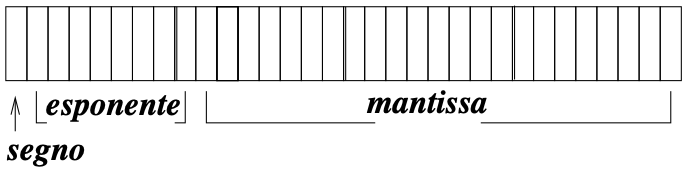
\includegraphics[width=0.5\linewidth]{images/IEEE.png}
    \centering
\end{figure}
\newpage
In precisione singola vengono destinati 24 bit alla mantissa (in realtà solo
23\footnote{Essendo sempre $\alpha_1$=1 per la rappresentazione binaria, la
prima cifra può essere sottintesa senza mai essere fisicamente memorizzata.}) e
8 all'esponente ($2^8=256=\omega-\lambda+1,\text{ con }\lambda=-127\text{ e
}\omega=128$), mentre in precisione doppia le cifre della mantissa sono 53
(memorizzati 52 bit) e dell'esponente 11 ($2^{11}=2048=\omega-\lambda+1,\text{
con }\lambda=-1023\text{ e }\omega=1024$).\\ 
Si osservi che l'esponente è memorizzato per traslazione (\textit{exponent
biased}) e che la costante di traslazione (\textit{bias}) è $-\lambda$. Quindi,
se $p$ è l'esponente del numero e $\tilde{p}$ è l'esponente memorizzato,
possiamo trovare l'esponente memorizzato a partire dall'esponente originale
utilizzando la seguente relazione:
$$\tilde{p}=p-\lambda$$
Dato un numero reale non nullo, $\alpha$, per associare un numero finito ad
esso, procediamo come segue:
\begin{enumerate}
    \item \textbf{Rappresentazione esatta}. Se $\alpha$ è scritto nella forma
        $\alpha=\pm(.\alpha_1\alpha_2\ldots)\times\beta^{p}$ tale che
        $\lambda\leq p\leq\omega$, $\alpha_i=0$ per $i> t$, allora è
        rappresentabile \underline{esattamente} come un numero finito $t$ di
        cifre e $\alpha\in \mathbb{F}(\beta,t,\lambda,\omega)$.
    \item \textbf{Rappresentazione approssimata}. Altrimenti 
        $\alpha\notin \mathbb{F}(\beta,t,\lambda,\omega)$ e quindi
        bisogna associargli un numero \underline{approssimato} $\tilde\alpha$
        che indicheremo con $fl(\alpha)$. Si hanno i seguenti casi:
        \begin{itemize}
            \item $p\notin[\lambda,\omega]$, viene segnalata una condizione
                d'errore:
                \begin{center}
                    \begin{tabular}{ll}
                        $p<\lambda$ & \textit{underflow} \\ 
                        $p>\lambda$ & \textit{overflow} \\ 
                   \end{tabular} 
                \end{center}
            \item $p\in[\lambda,\omega]$, ma le cifre $a_i$ con $i>t$ non sono
                tutte nulle, allora viene assegnato un numero finito $fl(\alpha)$
                seguendo due possibili criteri:
                \begin{itemize}
                    \item\textbf{Troncamento} di $\alpha$ alla t-esima cifra
                        $$fl_{T}(\alpha)=\pm(\sum_{i=1}^{t}\alpha_i\beta^{-i})\beta^p$$
                    \item\textbf{Arrotondamento} di $\alpha$ alla t-esima cifra 
                        $$fl_{A}(\alpha)=\pm
                        fl_{T}((\sum_{i=1}^{t+1}\alpha_i\beta^{-i}+\frac{\beta}{2}\beta^{-(t+1)})\beta^p)$$
                \end{itemize}
        \end{itemize}
\end{enumerate}
\begin{example}
    Il numero $\alpha=(0.11011)_2$ ha una mantissa di lunghezza 5, che è più
    lunga delle 3 cifre consentite in $\mathbb{F}(2,3,-1,2)$. Quindi, procediamo
    con l'operazione di arrotondamento:
    \begin{center}
       \begin{tabular}{lll}
           $fl_{A}(\alpha)=$ & $0.11011$ & + \\ 
                        & $0.00010$ & = \\ 
                        \hline
                        & $0.11100$ & \\ 
       \end{tabular} 
    \end{center}
\end{example}
\newpage
\begin{example}
   Consideriamo l'insieme dei numeri finiti $\mathbb{F}(10,5,-50,49)$. Per
   rappresentare un numero finito in questo insieme in memoria, dobbiamo
   definire il numero di posizioni necessarie. Nello specifico:
   \begin{itemize}
       \item\textbf{Segno}: una posizione è riservata per il segno. Se il numero
           è positivo si usa 0; se è negativo, si usa $\beta-1$.
        \item\textbf{Esponente}: due posizioni sono destinate all'esponente.
            Usando la tecnica di memorizzazione per traslazione
            ($p-\lambda=\tilde{p}$), possiamo
            rappresentare gli esponenti da -50 a 49 attraverso valori
            memorizzati da 00 a 99.
        \item\textbf{Mantissa}: cinque posizioni sono dedicate alla mantissa.
   \end{itemize}
   \begin{center}
        \begin{tabular}{ll}
            $\alpha=0.0532=0.532\cdot10^{-1}$ & $fl(\alpha)=04953200$\\ 
            $\alpha=-237141=-0.237141\cdot10^{6}$ & $fl(\alpha)=95623714$
        \end{tabular}
   \end{center}
\end{example}
\begin{oss}
    Siano $x$ ed $y$ due numeri $\in \mathbb{F}$ \underline{consecutivi}
    positivi. Sia $\alpha\in \mathbb{R}$ tale che $x\leq\alpha<y$. 
    \begin{center}
        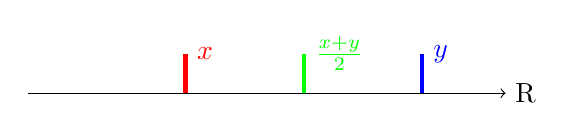
\begin{tikzpicture}
            \draw[->] (0,0) -- (0.5\linewidth,0) node[right] {R};

            \draw[red, ultra thick] (2,0) -- (2,0.5) node[right] {$x$};

            \draw[blue, ultra thick] (5,0) -- (5,0.5) node[right] {$y$};

            \draw[green, ultra thick] (3.5,0) -- (3.5,0.5) node[right] {$\frac{x+y}{2}$};
        \end{tikzpicture}
    \end{center}
    Allora possiamo affermare che $\alpha$ non appartiene all'insieme
    $\mathbb{F}$ perché, per ipotesi, $x$ e $y$ sono consecutivi e non ci può
    essere un altro numero tra loro. Tuttavia, la rappresentazione approssimata
    $fl(\alpha)$ risulta essere:
    \begin{center}
        \begin{tabular}{ll}
            $fl_T(\alpha)=x$ & $fl_A(\alpha)=\begin{cases}
                x & \text{se }\alpha<\frac{x+y}{2} \\ 
                y & \text{se }\alpha\geq \frac{x+y}{2}
            \end{cases}$
       \end{tabular} 
    \end{center}
    L'errore commesso nel troncamento sarà sempre maggiore o uguale dell'errore
    commesso nell'arrotondamento. Questo è il motivo per cui, con una base
    numerica pari, si preferisce utilizzare l'arrotondamento, poiché fornirà una
    migliore approssimazione del numero reale rispetto al troncamento.
\end{oss}
La modalità di arrotondamento dello standard ANSI/IEEE-754 coincide con quella
precedentemente descritta, con la particolarità dell'\textbf{arrotondamento ai
pari}. Questa particolarità si applica quando un numero reale $\alpha$ è esattamente 
equidistante dai numeri finiti consecutivi $x$ ed $y$, in altre parole, 
quando $\alpha=\frac{x+y}{2}$. In questa situazione l'arrotondamento funziona
nel seguente modo:
$$fl_{AP}(\alpha)=\begin{cases}
    x & \text{se }$x$\text{ è pari}\\ 
    $y$ & \text{se }$y$\text{ è pari}
\end{cases}$$
Sempre parlando dello standard ANSI/IEEE-754, per gestire risultati non rappresentabili, 
vengono utilizzati due valori speciali:
\begin{itemize}
    \item \textbf{NaN} 
    \item \textbf{Inf}
\end{itemize}
Invece, di avere un buco vicino allo zero dove i numeri molto piccoli
verrebbero immediatamente arrotondati a zero, vengono inseriti dei numeri ulteriori per
riempire questo buco e permettere ai valori di avvicinarsi progressivamente a zero.
Questo meccanismo è chiamato \textbf{gradual underflow}.\\ 
Per rappresentare questi numeri estremamente piccoli, si fa uso della
rappresentazione \textbf{denormalizzata}. In questa rappresentazione, la
mantissa  non inizia con il solito bit implicito di 1, ma  con una serie di 0.
\begin{example}
    Si eseguano i passi necessari per rappresentare il numero reale
    $(-13.9)_{10}$ in un'area di memoria di 8 bit (1 per il segno, 3 per
    l'exponent biased e 4 per la mantissa), che permettono di memorizzare
    $\mathbb{F}(2,5,-3,4)$ per troncamento e arrotondamento.
    \vskip 0.1in
    \begin{enumerate}
        \item \textbf{Conversione in binario}, prima la parte intera, quindi la parte decimale:
            \begin{itemize}
                \item \textit{Parte intera}:
                    \begin{enumerate}
                        \item Dividi il numero per 2.
                        \item Registra il resto della divisione (sarà 0 o 1).
                        \item Usa il quoziente ottenuto come nuovo numero e
                            ripeti la divisione per 2.
                        \item Continua il processo fino a quando il quoziente
                            diventa 0.
                        \item Leggi i resti della divisione in ordine
                            \underline{inverso}:
                            questo sarà il numero in base 2 della parte
                            intera.
                    \end{enumerate}
                    $$(13)_{10}=(1101)_2$$
                \item \textit{Parte decimale}:
                    \begin{enumerate}
                        \item Moltiplica la parte decimale per 2.
                        \item Registra la parte intera del risultato (sarà 0 o
                            1).
                        \item Usa la parte decimale del risultato come nuovo
                            numero e ripeti la moltiplicazione per 2.
                        \item Continua questo processo finché non ottieni una
                            parte decimale di 0 o si arriva al limite di
                            precisione della mantissa.
                        \item Leggi i numeri interi in ordine di apparizione:
                            questo sarà il numero in base 2 della parte
                            decimale.
                    \end{enumerate}
                    $$0.9\times2=\underline{1}.8$$
                    $$0.8\times2=\underline{1}.6$$
                    $$0.6\times2=\underline{1}.2$$
                    $$0.2\times2=\underline{0}.4$$
                    $$0.4\times2=\underline{0}.8$$
                    $$(0.9)_{10}=(11100\ldots)_2$$
            \end{itemize}
            da cui
            $$(-13.9)_{10}=(-1101.11100\ldots)_2$$
        \item \textbf{Normalizzazione}:
        nello standard IEEE-754, la rappresentazione normalizzata dei numeri
        in virgola mobile prevede che la parte \underline{intera} sia sempre
        1.
            $$(-1101.11100\ldots)_2=(-1.10111100\ldots)_2\times2^{3}$$
        \item \textbf{Calcolo dell'esponente biased}:
            $$p-\lambda=\tilde{p}\rightarrow3-(-3)=6$$
            $$(-1.10111100\ldots)_2\times2^3=(-1.10111100\ldots)_2\times2^{(110)_2}$$
        \item \textbf{Rappresentazione della mantissa}:
            \begin{center}
               \begin{tabular}{cc}
                    arrotondamento & troncamento \\ 
                   1.10111 + 0.00001 = 1.1100 & 1.1011
               \end{tabular} 
            \end{center}
        \item \textbf{Rappresentazione in memoria}: nello standard IEEE-754,
        con una mantissa di 5 bit, solo 4 bit vengono effettivamente memorizzati in memoria.
        \begin{center}
           \begin{tabular}{cc}
               $
               \begin{array}{|c|c|c|c|c|c|c|c|}
                   \hline
                   1 & 1 & 1 & 0 & 1 & 1 & 0 & 0\\
                   \hline
               \end{array} 
               $ 
                &
                $
                \begin{array}{|c|c|c|c|c|c|c|c|}
                    \hline
                    1 & 1 & 1 & 0 & 1 & 0 & 1 & 1 \\
                    \hline
                \end{array}
                $
           \end{tabular} 
        \end{center}
    \end{enumerate}
\end{example}
\subsection{Errori di rappresentazione}
\begin{definition}\leavevmode\
    Consideriamo un valore $\alpha\in \mathbb{R}$. Se $\alpha\notin
    \mathbb{F}(\beta,t,\lambda,\omega)$, allora la sua migliore
    approssimazione all'interno di questo insieme è data da $\tilde\alpha\in
    \mathbb{F}(\beta,t,\lambda,\omega)$. L'approssimazione di $\alpha$ con
    $\tilde\alpha$ introduce un \textbf{errore di rappresentazione}. Per quantificare
    tale errore, definiamo le seguenti metriche:
    {
        \renewcommand{\arraystretch}{1.5}
        \begin{center}
           \begin{tabular}{ll}
                $E_{abs}=\lvert \alpha-fl(\alpha)\rvert$ & errore assoluto \\
                $E_{rel}=\lvert \frac{\alpha-fl(\alpha)}{\alpha}\rvert\text{ se
            }\alpha\neq0$ & errore relativo 
           \end{tabular}
        \end{center}
    }
\end{definition}
Nel calcolo scientifico, l'errore relativo è preferito poiché fornisce una
misura dell'errore ``normalizzata'', che non dipende dalla grandezza dei numeri confrontati.
\begin{example}
    Si converta quanto rappresentato nell'esempio precedente nuovamente in
    base 10. Successivamente, si valuti l'errore assoluto e l'errore relativo
    della rappresentazione.
    \begin{enumerate}
        \setcounter{enumi}{5}
        \item\textbf{Decodifica}: per riconvertire il numero floating point
            appena determinato, faremo:
            \begin{center}
                 \begin{tabular}{ll}
                     arrotondamento & troncamento \\ 
                     $(-1.1100)_2\times2^{(110)_2}$ & $(-1.1011)_2\times2^{(110)_2}$ \\ 
                     $(-1.1100)_2\times2^{(3)_{10}}$ & $(-1.1011)_2\times2^{(3)_{10}}$ \\ 
                     $(-1110.0)_2$ & $(-1101.1)_2$ \\ 
                     $-(8+4+2+0+0)_{10}$ & $-(8+4+0+1+0.5)_{10}$ \\ 
                     $-(14)_{10}$ & $-(13.5)_{10}$ \\ 
                 \end{tabular}
            \end{center}
            \begin{center}
                \begin{tabular}{l|l|l}
                    & arrotondamento & troncamento \\
                    \hline
                    errore assoluto & $-13.9 - (-14) = 0.1$ & $-13.9 - (-13.5) = -0.4$ \\
                    \hline
                    errore relativo & $\frac{0.1}{-13.9} = -0.0072$ & $\frac{-0.4}{-13.9} = 0.0288$
                \end{tabular} 
            \end{center}
   \end{enumerate} 
\end{example}
\begin{definition}
    Dato l'insieme dei numeri finiti $\mathbb{F}(\beta,t,\lambda,\omega)$, si
    dice \textbf{unità di arrotondamento} e la si indica con $u$, la quantità:
    $$u=\begin{cases}
        \beta^{1-t} & \text{per troncamento} \\ 
        \frac{1}{2}\beta^{1-t} & \text{per arrotondamento}
    \end{cases}$$
\end{definition}
\begin{theorem}
   Per ogni $\alpha\in \mathbb{R}$ e $\alpha\notin0$ vale
   $$\Big\lvert \frac{\alpha-fl(\alpha)}{\alpha}\Big\rvert=u$$
\end{theorem}
Il teorema afferma che $u$, l'unità di arrotondamento, rappresenta il
\underline{limite superiore} dell'errore relativo quando si rappresenta 
un numero reale in un formato numerico finito.
\begin{example}
    Consideriamo l'insieme dei numeri finiti $\mathbb{F}(2,5,-3,4)$. Calcolare l'unità di arrotondamento $u$ sia nel caso di troncamento che di
    arrotondamento.
    $$u=\begin{cases}
        2^{1-5}=\frac{1}{16}=0.0625 & \text{per
        troncamento} \\
        \frac{1}{2}\cdot2^{1-5}=\frac{1}{32}=0.0325 & \text{per arrotondamento}
    \end{cases}$$
\end{example}
Indicheremo con $\epsilon$ l'errore relativo.
\begin{corollary}
    Per ogni $\alpha\in \mathbb{R}$ e $\alpha\notin0$ vale 
    $$  fl(\alpha)=\alpha(1\pm\epsilon),\quad \text{con }\lvert 
      \epsilon\rvert<u $$
\end{corollary} 
\begin{proof}\leavevmode\\
    Banalmente dato $\epsilon=\frac{\alpha-fl(\alpha)}{\alpha}$,
    per il Teorema si ha che $\lvert \epsilon\rvert<u$ e
    $fl(\alpha)=\alpha\epsilon+\alpha=\alpha(1+\epsilon)$.
\end{proof}
\paragraph{Precisione desiderata in base 10.}
La questione chiave è: quante cifre in base 10 sono necessarie per
rappresentare con precisione ciò che è memorizzato in base 2? 

Supponiamo di avere un numero rappresentato con $t$ cifre in base 2. Vogliamo
sapere a quante cifre, $s$, in base 10 questo corrisponde.

Partendo dall'equazione:
$$2^{-t}=10^{-s}$$
e applicando il logaritmo in base 10 ad entrambi i lati:
$$-t\times\log_{10}(2)=-s$$
da qui possiamo isolare $s$:
$$s=t\times\log_{10}(2)$$
usando un'approssimazione per il logaritmo:
$$s \approx t \times 0.30103$$

Per esempio:
\begin{itemize}
\item Nella precisione `basic single', con \( t = 24 \) cifre in base 2 per la mantissa, abbiamo:
$$s \approx 24 \times 0.30103 \approx 7.224$$
\item Nella precisione `basic double', con \( t = 53 \) cifre in base 2 per la mantissa, abbiamo:
$$s \approx 53 \times 0.30103 \approx 15.95459$$
\end{itemize}
Questo indica che ci servono circa 7-8 cifre in `basic single' o circa 16
cifre in `basic double' in base 10 per rappresentare con
precisione ciò che è memorizzato in base 2. Utilizzando meno cifre, stiamo
arrotondando e potremmo perdere informazioni.

Possiamo calcolare l'unità di arrotondamento $u$ per `basic single' e `basic
double':
\begin{itemize}
    \item $u_{single}= \frac{1}{2} \times 2^{1-24}=2^-24\approx 5.96 \times
        10 ^{-8}$ 
    \item $u_{double}= \frac{1}{2} \times 2^{1-53}=2^-53\approx 1.116 \times
        10 ^{-16}$ 
\end{itemize}
Ora, se confrontiamo questi valori con le cifre necessarie in base 10 per
una rappresentazione accurata, notiamo una relazione. Le cifre necessarie
sono legate all'ordine di grandezza dell'unità di arrotondamento.

Questi valori forniscono un indicatore sull'ordine di grandezza minimo dei 
numeri che possono essere rappresentati accuratamente e sul numero massimo di 
cifre che possiamo stampare senza perdere informazioni.
\subsection{Aritmetica finita}
Dati due numeri $a$ e $b$ appartenenti a $\mathbb{F}(\beta,t,\lambda,\omega)$,
l'operazione $a\ op\ b$ potrebbe produrre un risultato che non è contenuto in
$\mathbb{F}(\beta,t,\lambda,\omega)$.
\begin{example}
    Siano $a=(0.34)_{10}\times10^{0}$ e $b=(0.12)_{10}\times10^{-2}\in
    \mathbb{F}(10,2,\lambda,\omega)$. Eseguendo la somma si ha: 
    $$0.34+0.0012=0.3412$$
    ma, $0.3412\notin \mathbb{F}(10,2,\lambda,\omega)$.
\end{example}
Per eseguire le operazioni in questo dominio, vengono definiti degli
operatori specifici, che indichiamo con $\tilde{op}$ (ad esempio, $\tilde{+},
\tilde{-}, \tilde{*}, \tilde{/}$).
\begin{definition}
    L'operatore $\tilde{op}$ tra due numeri $a,b\in \mathbb{F}$ è definito nel modo seguente:
    $$a\ \tilde{op}\ b=fl(a\ op\ b)$$
    Questo significa che viene prima eseguita l'operazione in aritmetica
    esatta, e il risultato viene arrotondato per rientrare nell'insieme di
    numeri finiti $\mathbb{F}$.
\end{definition}
Per soddisfare tali requisiti, si utilizzano dei registri posizionati vicino 
al processore. Questi registri, dotati di bit aggiuntivi, 
rispetto a quelli della mantissa, permettono di eseguire operazioni con una
precisione superiore rispetto a quella raggiungibile con solo $t$ bit. Tale
maggiore precisione assicura che, arrotondando a $t$ cifre, il risultato ottenuto
aderisce alla definizione delineata sopra. Idealmente, un registro di lunghezza
$t+1$ bit, superiore a quella della mantissa stessa, garantirebbe la
conformità a questa definizione.
\vskip 0.1in
\paragraph{Errore in aritmetica finita.}
Qual'è l'errore massimo che possiamo commettere durante un operazione con numeri
finiti?
Consideriamo l'errore relativo tra il risultato ottenuto in aritmetica finita
e quello in aritmetica esatta, si può notare un interessante comportamento. 
Notiamo che, il risultato esatto di $(a\ op\ b)$ è un numero $\alpha\in
\mathbb{R}$. Per definizione, in aritmetica finita, $(a\ \tilde{op}\ b)$ è
l'approssimazione floating-point di $\alpha$.
Allora, per il teorema sopra menzionato, possiamo dedurre che l'errore relativo massimo tra
$\alpha$ e $fl(\alpha)$ è minore dell'unità di arrotondamento $u$. Questo
significa che $u$ rappresenta l'errore relativo massimo che possiamo
aspettarci in una singola operazione in aritmetica finita.
Estendendo questa logica, se effettuiamo una serie di $n$ operazioni, l'errore
totale potrebbe essere al più $nu$.
$$\Big\lvert \frac{\overset{fl(\alpha)}{\overbrace{(a\ \tilde{op}\ b)}}-\overset{\alpha}{\overbrace{(a\ op\
b)}}}{\underset{\alpha}{\underbrace{a\ op\ b}}}\Big\rvert<u$$
\paragraph{Proprietà associativa.} La proprietà associativa afferma che
l'ordine in cui si raggruppano i termini durante un'operazione non modifica il
risultato. Tuttavia, essa, così come le altre proprietà, \underline{non} vale nell'aritmetica finita.
\begin{example}
    Considerati $a=0.11\times10^0,b=0.13\times10^{-1},c=0.14\times10^{-1}\in
    \mathbb{F}(10,2,\lambda,\omega)$.
    Verificare se la proprietà associativa
    $(a\tilde+b)\tilde+c=a\tilde+(b\tilde+c)$ è valida.
    \begin{equation*}
        \begin{aligned}
            (0.11\tilde+0.013)\tilde+0.014&=0.11\tilde+(0.013\tilde+0.014) \\ 
            fl(0.123)\tilde+0.014&=0.11\tilde+fl(0.027)\\ 
            0.12\tilde+0.014&=0.11\tilde+0.03 \\ 
            fl(0.134)&=0.14 \\
            0.13\times10^0&\neq0.14\times10^0
        \end{aligned} 
    \end{equation*}
    Concludendo, la proprietà associativa non è valida nell'ambito dell'aritmetica finita.
\end{example}
Questo significa che la stessa istruzione o espressione, se scritta in modi
diversi, può produrre risultati differenti. 
Di conseguenza, è importante comprendere come evitare di scrivere operazioni che
potrebbero causare errori più grandi.
\subsubsection{Caratterizzazione di $u$}
L'unità di arrotondamento $u$ ha un'importanza numerica sia in relazione alla precisione
di rappresentazione (Teorema) che in termini di precisione di calcolo (risultato precedente).
La sua importanza numerica è ulteriormente sottolineata dalla seguente
caratterizzazione:

\begin{center}
    \emph{$u$ è il più piccolo numero finito positivo tale che, se sommato a
    1, viene ``sentito'' e risulta essere $>$ di 1.}
\end{center}
$$u\tilde+1>1$$
Questo implica che per ogni numero finito $v<u$ sarà $v\tilde+1=1$.

Infatti, se sommiamo un numero $v$ a $1$:
    $$
    \underbrace{1.0 \ldots 0}_{t \text{ cifre}} + \underbrace{0.0 \ldots 0}_{t
    \text{ cifre}}1
    $$
Tuttavia, il valore $1$ rimane fuori dalle $t$ cifre e nella somma viene
arrotondato, e non viene ``sentito'' poiché il risultato sarà comunque $1$.

\begin{center}
    \begin{tikzpicture}
        \draw[->] (-2,0) -- (2*5,0) node[right] {R};
        \draw (0,0.1) -- (0,-0.1) node[below] {0};
        \draw[blue] (1,0) -- (1,-0.4) node[below] {$u\tilde+1>1$};
        \draw[red] (1,0) -- (1,0.4) node[above] {$v\tilde+1$=1};
        \draw[blue] (1,-0.4) -- (2*3.5,-0.4);
        \draw[red] (1,0.4) -- (0,0.4);
        \draw[dashed, blue] (2*3.5,-0.4) -- (2*4,-0.4);
        \filldraw (0,0) circle (0.05);

        \foreach \x in {0.25, 0.3125, 0.375, 0.4375, 0.625, 0.75, 0.875, 1, 1.25, 1.5, 1.75, 2, 2.5, 3, 3.5} {
            \draw (2*\x,-0.1) -- (2*\x,0.1);
        }
    \end{tikzpicture}
\end{center}
Invece, se sommiamo un numero $u$ a 1:
\begin{equation*}
   \begin{aligned}
       u\tilde+1&=\frac{1}{2}\beta^{1-t}+1 \\ 
                &=\frac{\beta}{2}\beta^{-t}+1 \\
                &=0.0\ldots0\frac{\beta}{2}+\underbrace{1.0\ldots0}_{t\text{
                cifre}} \\ 
                &= 1.0\ldots0 \frac{\beta}{2}+0.0+0.0\ldots0 \frac{\beta}{2}
                \text{ per arrotondamento}\\
                &= \underbrace{1.0\ldots1}_{t\text{ cifre}}0 \text{ per
                troncamento}\\
                1.0\ldots1&>1
   \end{aligned} 
\end{equation*}
Nello standard IEEE-754, se consideriamo l'arrotondamento ai pari e dato che
$1.0\ldots0 \frac{\beta}{2}=\frac{x+y}{2}$, dove $x=1$ e
$y=1.0\ldots1$, il valore pari più vicino è 1. Pertanto, 1 verrà scelto come
risultato dell'arrotondamento. Questo cambia la caratterizzazione di $u$:
\begin{center}
    \emph{$u$ è il più grande numero finito positivo tale che, se sommato a 1,
    risulta essere $=1$}.
\end{center}
$$u\tilde+1=1$$
\begin{center}
    \begin{tikzpicture}
        \draw[->] (-2,0) -- (2*5,0) node[right] {R};
        \draw (0,0.1) -- (0,-0.1) node[below] {0};
        \draw[red] (1,0) -- (1,-0.4) node[below] {$v\tilde+1>1$};
        \draw[blue] (1,0) -- (1,0.4) node[above] {$u\tilde+1$=1};
        \draw[red] (1,-0.4) -- (2*3.5,-0.4);
        \draw[blue] (1,0.4) -- (0,0.4);
        \draw[dashed, red] (2*3.5,-0.4) -- (2*4,-0.4);
        \filldraw (0,0) circle (0.05);

        \foreach \x in {0.25, 0.3125, 0.375, 0.4375, 0.625, 0.75, 0.875, 1, 1.25, 1.5, 1.75, 2, 2.5, 3, 3.5} {
            \draw (2*\x,-0.1) -- (2*\x,0.1);
        }
    \end{tikzpicture}
\end{center}
Ma cosa ci serve tutto a questo? Per determinare proceduralmente $u$:
\begin{enumerate}
    \item Esaminare le potenze negative di 2.
    \item Continuare finché non si individua una potenza $2^{-t}$ che, quando sommata a 1,
        produce come risultato esattamente 1.
    \item Tale potenza $2^{-t}$ rappresenta l'unità di arrotondamento $u$.
\end{enumerate}
\begin{verbatim}
    u=1
    t=0
    while (u+1>1)
        u=u/2
        t=t+1
    end 
    stampa(u,t)
\end{verbatim}
\end{document}
